\documentclass[letter,11pt]{article}

\usepackage[spanish,es-nodecimaldot]{babel}
\usepackage[utf8]{inputenc}

\usepackage{lmodern}
\usepackage[T1]{fontenc}
\usepackage{textcomp}

\usepackage{framed}
\usepackage[svgnames]{xcolor}
\colorlet{shadecolor}{Gainsboro!50}

\usepackage{graphicx}
\usepackage{pstricks}

\usepackage{anysize}
\marginsize{3cm}{2cm}{2cm}{3cm}

\usepackage{siunitx}
\usepackage{amsmath}
\usepackage{array}

\usepackage{fancyhdr}
\usepackage{lastpage}
\pagestyle{fancy}
\fancyhf{}
\fancyhead[LE,RO]{Física Básica III}
\fancyfoot[CO,CE]{\thepage\ de \pageref{LastPage}}

\special{papersize=215.9mm,279.4mm}

\usepackage[
    pdfauthor={Carlos Eduardo Caballero Burgoa},%
    pdftitle={Física Básica III},%
    pdfsubject={1er Parcial},%
    colorlinks,%
    citecolor=black,%
    filecolor=black,%
    linkcolor=black,%
    urlcolor=black,
    breaklinks]{hyperref}
\usepackage{breakurl}

\newcommand{\blankpage}{
\newpage
\thispagestyle{empty}
\mbox{}
\newpage
}

\renewcommand{\arraystretch}{1.2}

\begin{document}

\begin{center}
    {\Large \bf{Primer parcial}}
\end{center}

\noindent\fbox{%
    \parbox{\textwidth}{%
        Estudiante: CABALLERO BURGOA, Carlos Eduardo \\
        Carrera: Ingeniería Electromecánica \\
        Correo: cijkb.j@gmail.com
    }%
}

\vspace{0.5cm}

\begin{enumerate}
\item Una varilla delgada de longitud $2L$ ($L = 1 [m]$) y uniformemente cargada
por unidad de longitud ($\lambda = 1 [\mu C/m]$), yace a lo largo del eje $x$,
como se muestra en la figura. Calcular el campo eléctrico en el punto $P$, a una
distancia $d = 1 [m]$ de la varilla a lo largo de su bisectriz perpendicular.

\begin{figure}[!h]
\centering
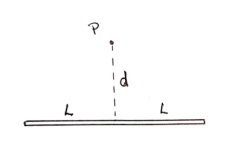
\includegraphics[scale=1.60]{resources/q1.eps}
\end{figure}

\begin{itemize}
    \item \textcolor{red}{$12727.92 [N/C]$.}
    \item $11462.36 [N/C]$.
    \item $10354.28 [N/C]$.
    \item $ 9658.33 [N/C]$.
\end{itemize}

\textbf{Solución:} \\

\begin{figure}[!h]
\centering
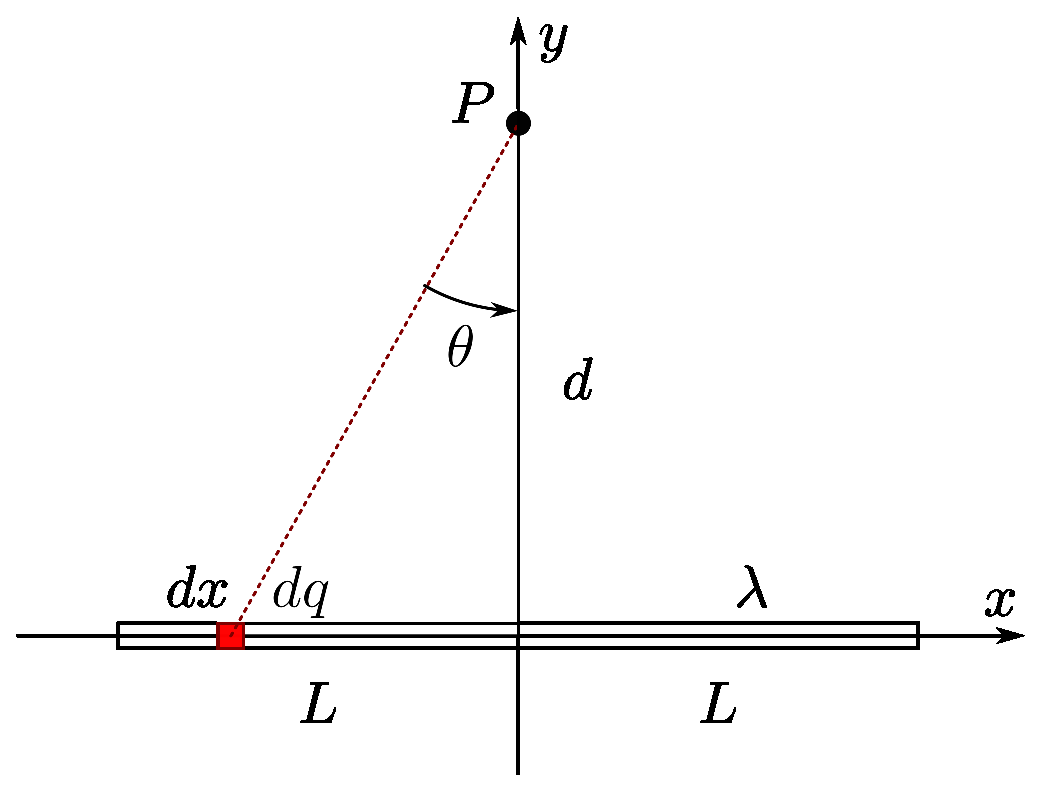
\includegraphics[scale=0.39]{resources/a1.eps}
\end{figure}

Dada la ecuación campo eléctrico:

\begin{equation*}
    \vec{E} = \frac{1}{4\pi\epsilon_0}\int_{Q}\frac{dq}{\vec{r}^2}
\end{equation*}

Y considerando la uniformidad de la carga:

\begin{equation*}
    \lambda = \frac{dq}{dx}
\end{equation*}

Entonces:

\begin{equation*}
    E_x = \frac{1}{4\pi\epsilon_0}\int_{-L}^{L}\frac{\lambda dx}{x^2+d^2}\,sen(\theta)
        = \frac{\lambda}{4\pi\epsilon_0}\int_{-L}^{L}\frac{dx}{x^2+d^2}\frac{x}{\sqrt{x^2+d^2}}
\end{equation*}
\begin{equation*}
    E_x = \frac{\lambda}{4\pi\epsilon_0}\int_{-L}^{L}\frac{x}{(x^2+d^2)^{3/2}}dx
        = \frac{\lambda}{4\pi\epsilon_0}\left(-\frac{1}{\sqrt{x^2+d^2}}\Biggr|_{-L}^{L}\right)
        = 0
\end{equation*}
\begin{equation*}
    E_y = \frac{1}{4\pi\epsilon_0}\int_{-L}^{L}\frac{\lambda dx}{x^2+d^2}\,cos(\theta)
        = \frac{\lambda}{4\pi\epsilon_0}\int_{-L}^{L}\frac{dx}{x^2+d^2}\frac{d}{\sqrt{x^2+d^2}}
\end{equation*}
\begin{equation*}
    E_y = \frac{\lambda\,d}{4\pi\epsilon_0}\int_{-L}^{L}\frac{1}{(x^2+d^2)^{3/2}}dx
        = \frac{\lambda}{4\pi\epsilon_0}\left(\frac{1}{d^2}\frac{x}{\sqrt{x^2+d^2}}\Biggr|_{-L}^{L}\right)
\end{equation*}
\begin{equation*}
    E_y = \frac{\lambda}{4\pi\epsilon_0}\left(\frac{2}{d^2}\frac{L}{\sqrt{L^2+d^2}}\right)
        = \frac{1}{4\pi\epsilon_0}\frac{2L\lambda}{d^2\sqrt{L^2+d^2}}
        = 12710.32 [N/C]
\end{equation*}

\item Considere un cilindro hueco con una pared delgada uniformemente cargada
con una carga total $Q = 1 [\mu C]$, radio $R = 0.1 [m]$ y una longitud
$L = 1 [m]$. Determine el campo eléctrico en un punto del eje a una distancia
$d = 0.2 [m]$ del lado derecho del cilindro como se muestra en la figura.

\begin{figure}[!h]
\centering
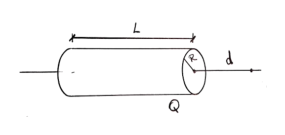
\includegraphics[scale=1.80]{resources/q2.eps}
\end{figure}

\begin{itemize}
    \item $41326.35 [N/C]$.
    \item \textcolor{red}{$32775.13 [N/C]$.}
    \item $25689.22 [N/C]$.
    \item $18567.46 [N/C]$.
\end{itemize}

\textbf{Solución:} \\

\begin{figure}[!h]
\centering
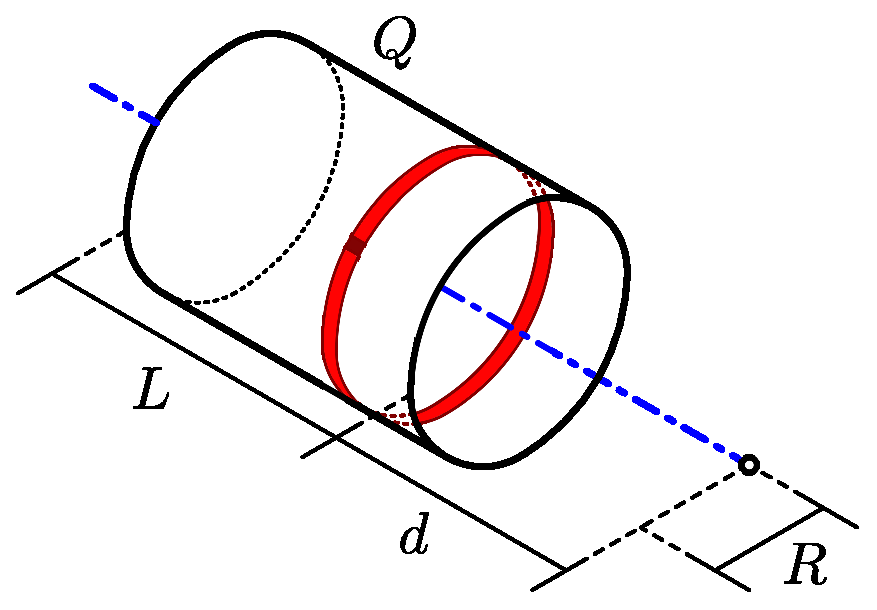
\includegraphics[scale=0.40]{resources/a2.eps}
\end{figure}

Dada la ecuación campo eléctrico:

\begin{equation*}
    \vec{E} = \frac{1}{4\pi\epsilon_0}\int_{Q}\frac{dq}{\vec{r}^2}
\end{equation*}

Y considerando la uniformidad de la carga:

\begin{equation*}
    \sigma = \frac{dq}{ds\,dx}
\end{equation*}

Entonces:

\begin{equation*}
    E_x = \frac{1}{4\pi\epsilon_0}\int_{d}^{d+L}\int_{0}^{2\pi\,R}\frac{\sigma\,ds\,dx}{x^2+R^2}\,cos(\theta)
        = \frac{\sigma}{4\pi\epsilon_0}\int_{d}^{d+L}\int_{0}^{2\pi\,R}\frac{ds\,dx}{x^2+R^2}\frac{x}{\sqrt{x^2+R^2}}
\end{equation*}
\begin{equation*}
    E_x = \frac{\sigma}{4\pi\epsilon_0}\int_{d}^{d+L}\int_{0}^{2\pi\,R}\frac{x\,ds\,dx}{(x^2+R^2)^{3/2}}
        = \frac{\sigma}{4\pi\epsilon_0}\int_{d}^{d+L}\frac{x}{(x^2+R^2)^{3/2}}dx\int_{0}^{2\pi\,R}ds
\end{equation*}
\begin{equation*}
    E_x = \frac{\sigma}{4\pi\epsilon_0}\int_{d}^{d+L}\frac{x\,dx}{(x^2+R^2)^{3/2}}(2\pi\,R)
        = \frac{\sigma R}{2\epsilon_0}\int_{d}^{d+L}\frac{x\,dx}{(x^2+R^2)^{3/2}}
\end{equation*}
\begin{equation*}
    E_x = \frac{\sigma R}{2\epsilon_0}\left(-\frac{1}{\sqrt{x^2+R^2}}\Biggr|_{d}^{d+L}\right)
        = \frac{\sigma R}{2\epsilon_0}\left(-\frac{1}{\sqrt{(d+L)^2+R^2}}+\frac{1}{\sqrt{d^2+R^2}}\right)
\end{equation*}

Reemplazando $\sigma = Q/2\pi\,R\,L$, obtenemos:

\begin{equation*}
    E = \frac{1}{4\pi\epsilon_0}\frac{Q}{L}\left(\frac{1}{\sqrt{d^2+R^2}}-\frac{1}{\sqrt{(d+L)^2+R^2}}\right)
      = 32729.7980 [N/C]
\end{equation*}

\item  Un cilindro aislante de longitud infinita y de radio $R = 0.3 [m]$, tiene
una densidad de carga volumétrica $\rho = \rho_0 (a - r/b )$ que varía en
función del radio donde: $\rho_0 = 1 [\mu C/m^3]$, $a = 4$, y $b = 2$ son
constantes positivas y $r$ es la distancia al eje del cilindro. Calcule la
magnitud del campo eléctrico en $r = 1 [m]$.

\begin{itemize}
    \item \textcolor{red}{$19830.51 [N/C]$.}
    \item $18575.46 [N/C]$.
    \item $17624.33 [N/C]$.
    \item $16458.29 [N/C]$.
\end{itemize}

\textbf{Solución:} \\

\begin{figure}[!h]
\centering
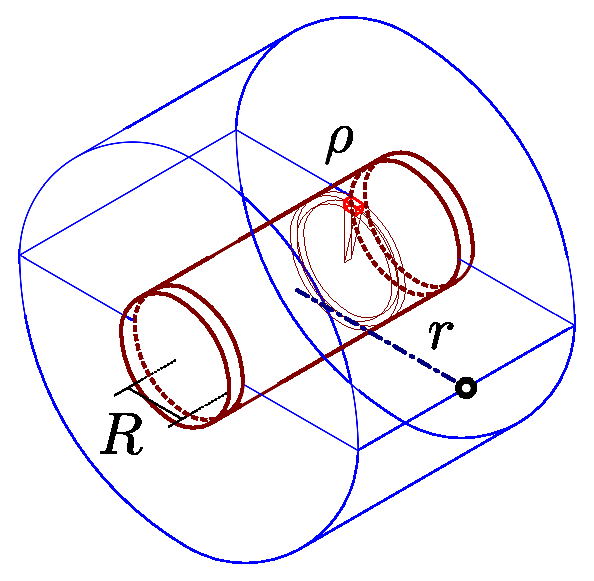
\includegraphics[scale=0.40]{resources/a3.eps}
\end{figure}

Usando la ley de \emph{Gauss}:

\begin{equation*}
    \Phi_E = \frac{Q_{enc}}{\epsilon_0}
\end{equation*}

Se halla la carga encerrada por la superficie gaussiana $Q_{enc}$ a partir
de la densidad volumétrica:

\begin{equation*}
    \rho = \frac{dq}{dV}
\end{equation*}
\begin{equation*}
    dq = \rho\,dV
\end{equation*}
\begin{equation*}
    dq = \rho\,r\,d\theta\,dr\,dL
\end{equation*}
\begin{equation*}
    dq = \rho_0\left(a-\frac{r}{b}\right)\,r\,d\theta\,dr\,dL
\end{equation*}
\begin{equation*}
    \int_{Q} dq = \int\int\int\rho_0\left(a-\frac{r}{b}\right)\,r\,d\theta\,dr\,dL
\end{equation*}
\begin{equation*}
    Q = \rho_0\int_{0}^{L}\int_{0}^{R}\int_{0}^{2\pi}\left(a-\frac{r}{b}\right)\,r\,d\theta\,dr\,dL
      = \rho_0\int_{0}^{L}\int_{0}^{R}\left(a-\frac{r}{b}\right)\,r\,2\pi\,dr\,dL
\end{equation*}
\begin{equation*}
    Q = 2\pi\,\rho_0\int_{0}^{L}\int_{0}^{R}\left(ar-\frac{r^2}{b}\right)\,dr\,dL
      = 2\pi\,\rho_0\int_{0}^{L}\left(\frac{ar^2}{2}-\frac{r^3}{3b}\right)\Biggr|_{0}^{R}dL
\end{equation*}
\begin{equation*}
    Q = 2\pi\,\rho_0\,\left(\frac{aR^2}{2}-\frac{R^3}{3b}\right)\int_{0}^{L}dL
      = 2\pi\,\rho_0\,\left(\frac{aR^2}{2}-\frac{R^3}{3b}\right)L
\end{equation*}
\begin{equation*}
   Q  = 2\pi\,\rho_0\,L\,\left(\frac{aR^2}{2}-\frac{R^3}{3b}\right)
\end{equation*}

Por tanto:

\begin{equation*}
    E_{\perp}\,A = \frac{Q_{enc}}{\epsilon_0}
\end{equation*}
\begin{equation*}
    E\,(2\pi\,r\,L) = \frac{1}{\epsilon_0}2\pi\,\rho_0\,L\,\left(\frac{aR^2}{2}-\frac{R^3}{3b}\right)
\end{equation*}
\begin{equation*}
    E = \frac{\rho_0}{\epsilon_0\,r}\,\left(\frac{aR^2}{2}-\frac{R^3}{3b}\right)
      = 19821,1291 [N/C]
\end{equation*}

\item Un alambre con una densidad lineal de carga uniforme igual a
$1 [\mu C/m]$, se dobla como se muestra en la figura. Calcular el potencial
eléctrico en el punto $0$.

\begin{figure}[!h]
\centering
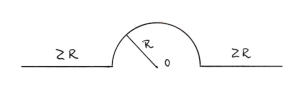
\includegraphics[scale=1.80]{resources/q4.eps}
\end{figure}

\begin{itemize}
    \item $43419.92 [V]$.
    \item $44603.85 [V]$.
    \item $46371.26 [V]$.
    \item \textcolor{red}{$48049.36 [V]$.}
\end{itemize}

\textbf{Solución:} \\

Se calcula el potencial separando el alambre en tres partes:

\begin{equation*}
    V = V_1+V_2+V_3
\end{equation*}

Conociendo la ecuación del potencial eléctrico:

\begin{equation*}
    V = \frac{1}{4\pi\epsilon_0}\int_{Q}\frac{dq}{r}
\end{equation*}

Para $V1$ y $V_3$:

Considerando una distribución lineal de carga:

\begin{equation*}
    \lambda = \frac{dq}{dx}
\end{equation*}
\begin{equation*}
    dq = \lambda\,dx
\end{equation*}

Se calcula el potencial eléctrico:

\begin{equation*}
    V = \frac{1}{4\pi\epsilon_0}\int_{Q}\frac{dq}{x}
      = \frac{1}{4\pi\epsilon_0}\int_{R}^{3R}\lambda\frac{dx}{x}
      = \frac{\lambda}{4\pi\epsilon_0}\left(ln x\Biggr|_{R}^{3R}\right)
      = \frac{\lambda}{4\pi\epsilon_0}(ln(3R)-ln(R))
\end{equation*}
\begin{equation*}
    V = \frac{\lambda}{4\pi\epsilon_0}\left(ln \frac{3R}{R}\right)
      = \frac{1}{4\pi\epsilon_0}\lambda\,ln(3)
\end{equation*}

Para $V3$:

Considerando una distribución lineal de carga:

\begin{equation*}
    \lambda = \frac{dq}{ds} = \frac{dq}{R\,d\theta}
\end{equation*}
\begin{equation*}
    dq = \lambda\,R\,d\theta
\end{equation*}

Se calcula el potencial eléctrico:

\begin{equation*}
    V = \frac{1}{4\pi\epsilon_0}\int_{Q}\frac{dq}{x}
      = \frac{1}{4\pi\epsilon_0}\int_{0}^{\pi}\lambda\frac{R\,d\theta}{R}
      = \frac{\lambda}{4\pi\epsilon_0}\int_{0}^{\pi}d\theta
      = \frac{1}{4\pi\epsilon_0}\lambda\,\pi
\end{equation*}

Por tanto:

\begin{equation*}
    V = \frac{1}{4\pi\epsilon_0}\lambda\,ln(3)
      + \frac{1}{4\pi\epsilon_0}\lambda\,\pi
      + \frac{1}{4\pi\epsilon_0}\lambda\,ln(3)
\end{equation*}
\begin{equation*}
    V = \frac{1}{4\pi\epsilon_0}\lambda(\pi+\,2\,ln(3))
      = 47982.8963 [V]
\end{equation*}

\item Un capacitor de placas paralelas de $2 [nF]$ se carga con una diferencia
de potencial de $100 [V]$ y se aísla (desconecta de la batería) a continuación.
El material dieléctrico que llevaba entre las placas es mica con una constante
dieléctrica de $5$. Calcular el trabajo que se requiere para retirar la hoja de
mica.

\begin{itemize}
    \item $38 [\mu J]$.
    \item $39 [\mu J]$.
    \item \textcolor{red}{$40 [\mu J]$.}
    \item $41 [\mu J]$.
\end{itemize}

\textbf{Solución:} \\

La energía almacenada en un capacitor es:

\begin{equation*}
    U = \frac{1}{2}CV^2
\end{equation*}

De la definición de $K$ del dieléctrico:

\begin{equation*}
    K = \frac{C}{C_0}
\end{equation*}
\begin{equation*}
    V = \frac{V_0}{K}
\end{equation*}

El trabajo requerido es la diferencia de energía del capacitor con y sin el
dieléctrico:

\begin{equation*}
    U = U_0 - U_D
      = \frac{1}{2}C_0\,V^2_0-\frac{1}{2}C\,V^2
      = \frac{1}{2}\left(\frac{C}{K}\right)(V\,K)^2-\frac{1}{2}C\,V^2
\end{equation*}
\begin{equation*}
    U = \frac{1}{2}\left(\frac{C}{K}\right)V^2\,K^2-\frac{1}{2}C\,V^2
      = \frac{1}{2}C\,V^2\,K+\frac{1}{2}C\,V^2
\end{equation*}
\begin{equation*}
    U = \frac{1}{2}C\,V^2(K-1) = \num{4e-5} [J] = 40 [\mu J]
\end{equation*}

\end{enumerate}

\end{document}

